\documentclass[a4paper]{article}

\usepackage[english]{babel}
\usepackage[utf8]{inputenc}
\usepackage{amsmath}
\usepackage{graphicx}
\usepackage[colorinlistoftodos]{todonotes}
\usepackage{caption}
\usepackage{subcaption}
\usepackage{here}

\title{Computational Photography \\ Project 1, Fall 2014}

\author{Mich\`ele Wyss, 10-104-123}

\date{October 2, 2014}

\graphicspath{{imgs/}}
\begin{document}
\maketitle
\section{The Spanish Castle illusion}
The Spanish Castle illusion is an astonishing effect to demonstrate how the human eye can be influenced by temporal effects.  In the 19$^{\text{th}}$ century, the so-called \emph{Opponent process theory} was proposed. According to this theory, the color perception of a human eye is controlled by ``encoding'' colors as red vs.\ green,  blue vs.\ yellow and blak vs.\ white. Further, the theory states that are two types of chemical reactions, namely \emph{anabolic} and \emph{catabolic} processes. For simplicity, one could understand them as ``positive'' or ``negative'' reactions. The processes are in a sense the opposite of each other. The positive reaction yields one member of an opponent pair, whereas the negative reaction yields the other one. An anabolic process requires energy and a catabolic one releases energy. If a stimulus of a certain color is given, then the corresponding process will be reversed after the stimulus is removed again, and this will give the impression of perceiving the opposite color.
\section*{Example images}
\begin{figure}[H]
	%\centering
	\begin{subfigure}[h]{0.24\textwidth}
		\centering
		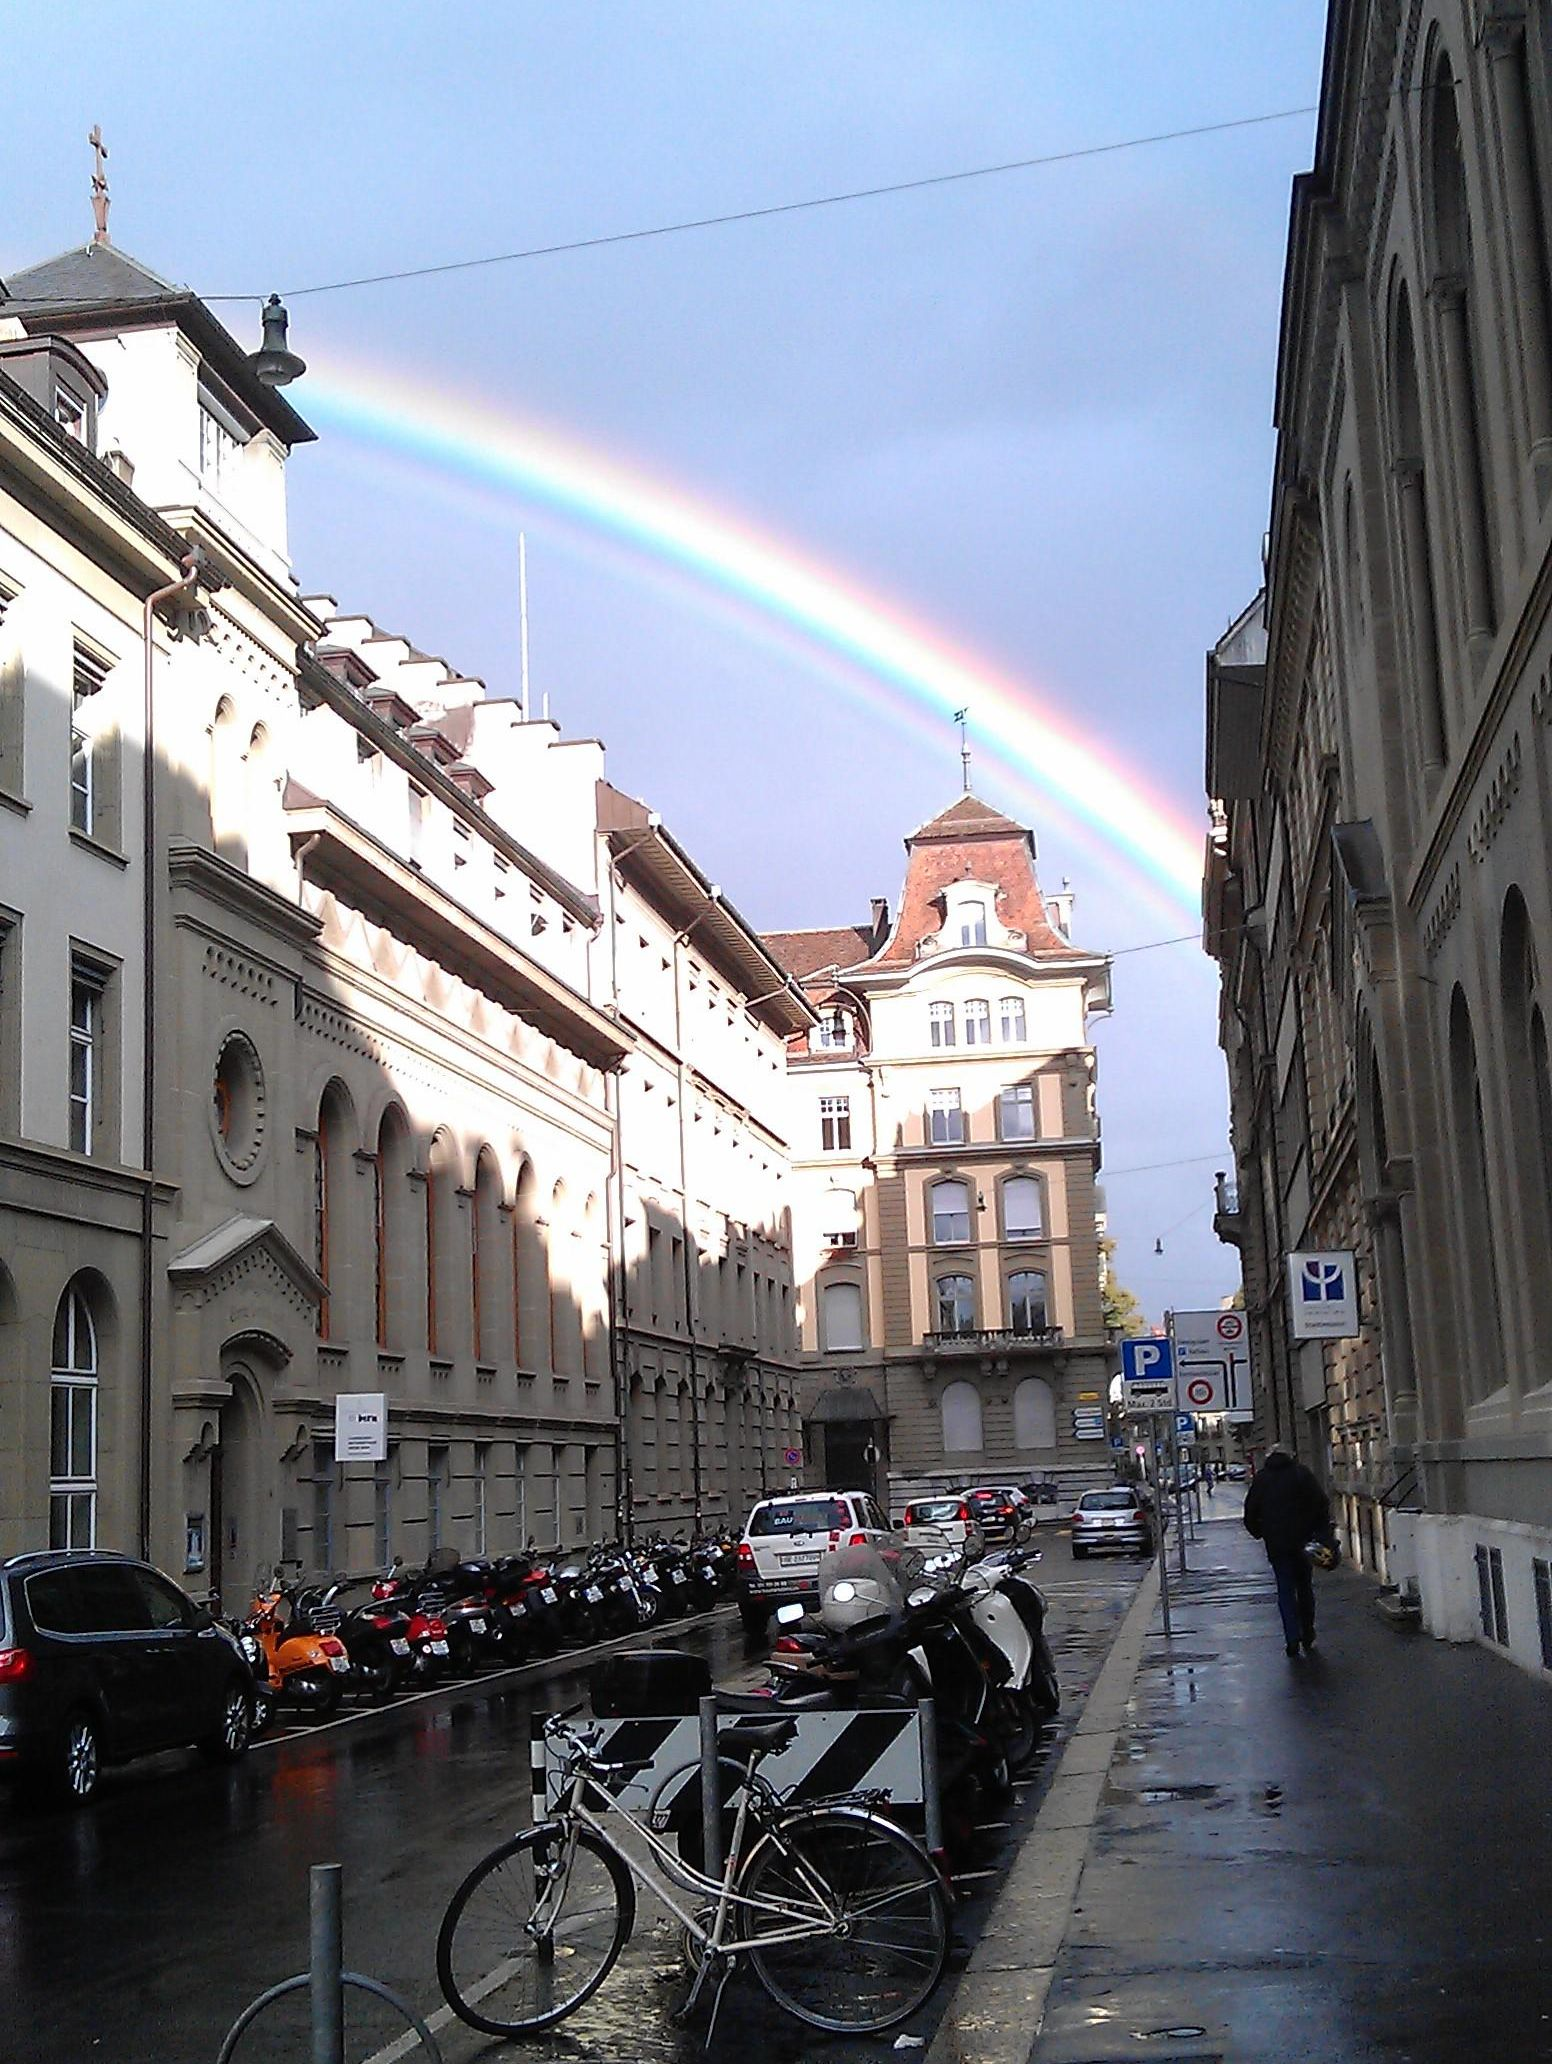
\includegraphics[width=\textwidth]{rainbow}
		\caption*{Input image}
	\end{subfigure}
	
	\vspace{3mm}
	\begin{subfigure}[h]{0.48\textwidth}
		\centering
		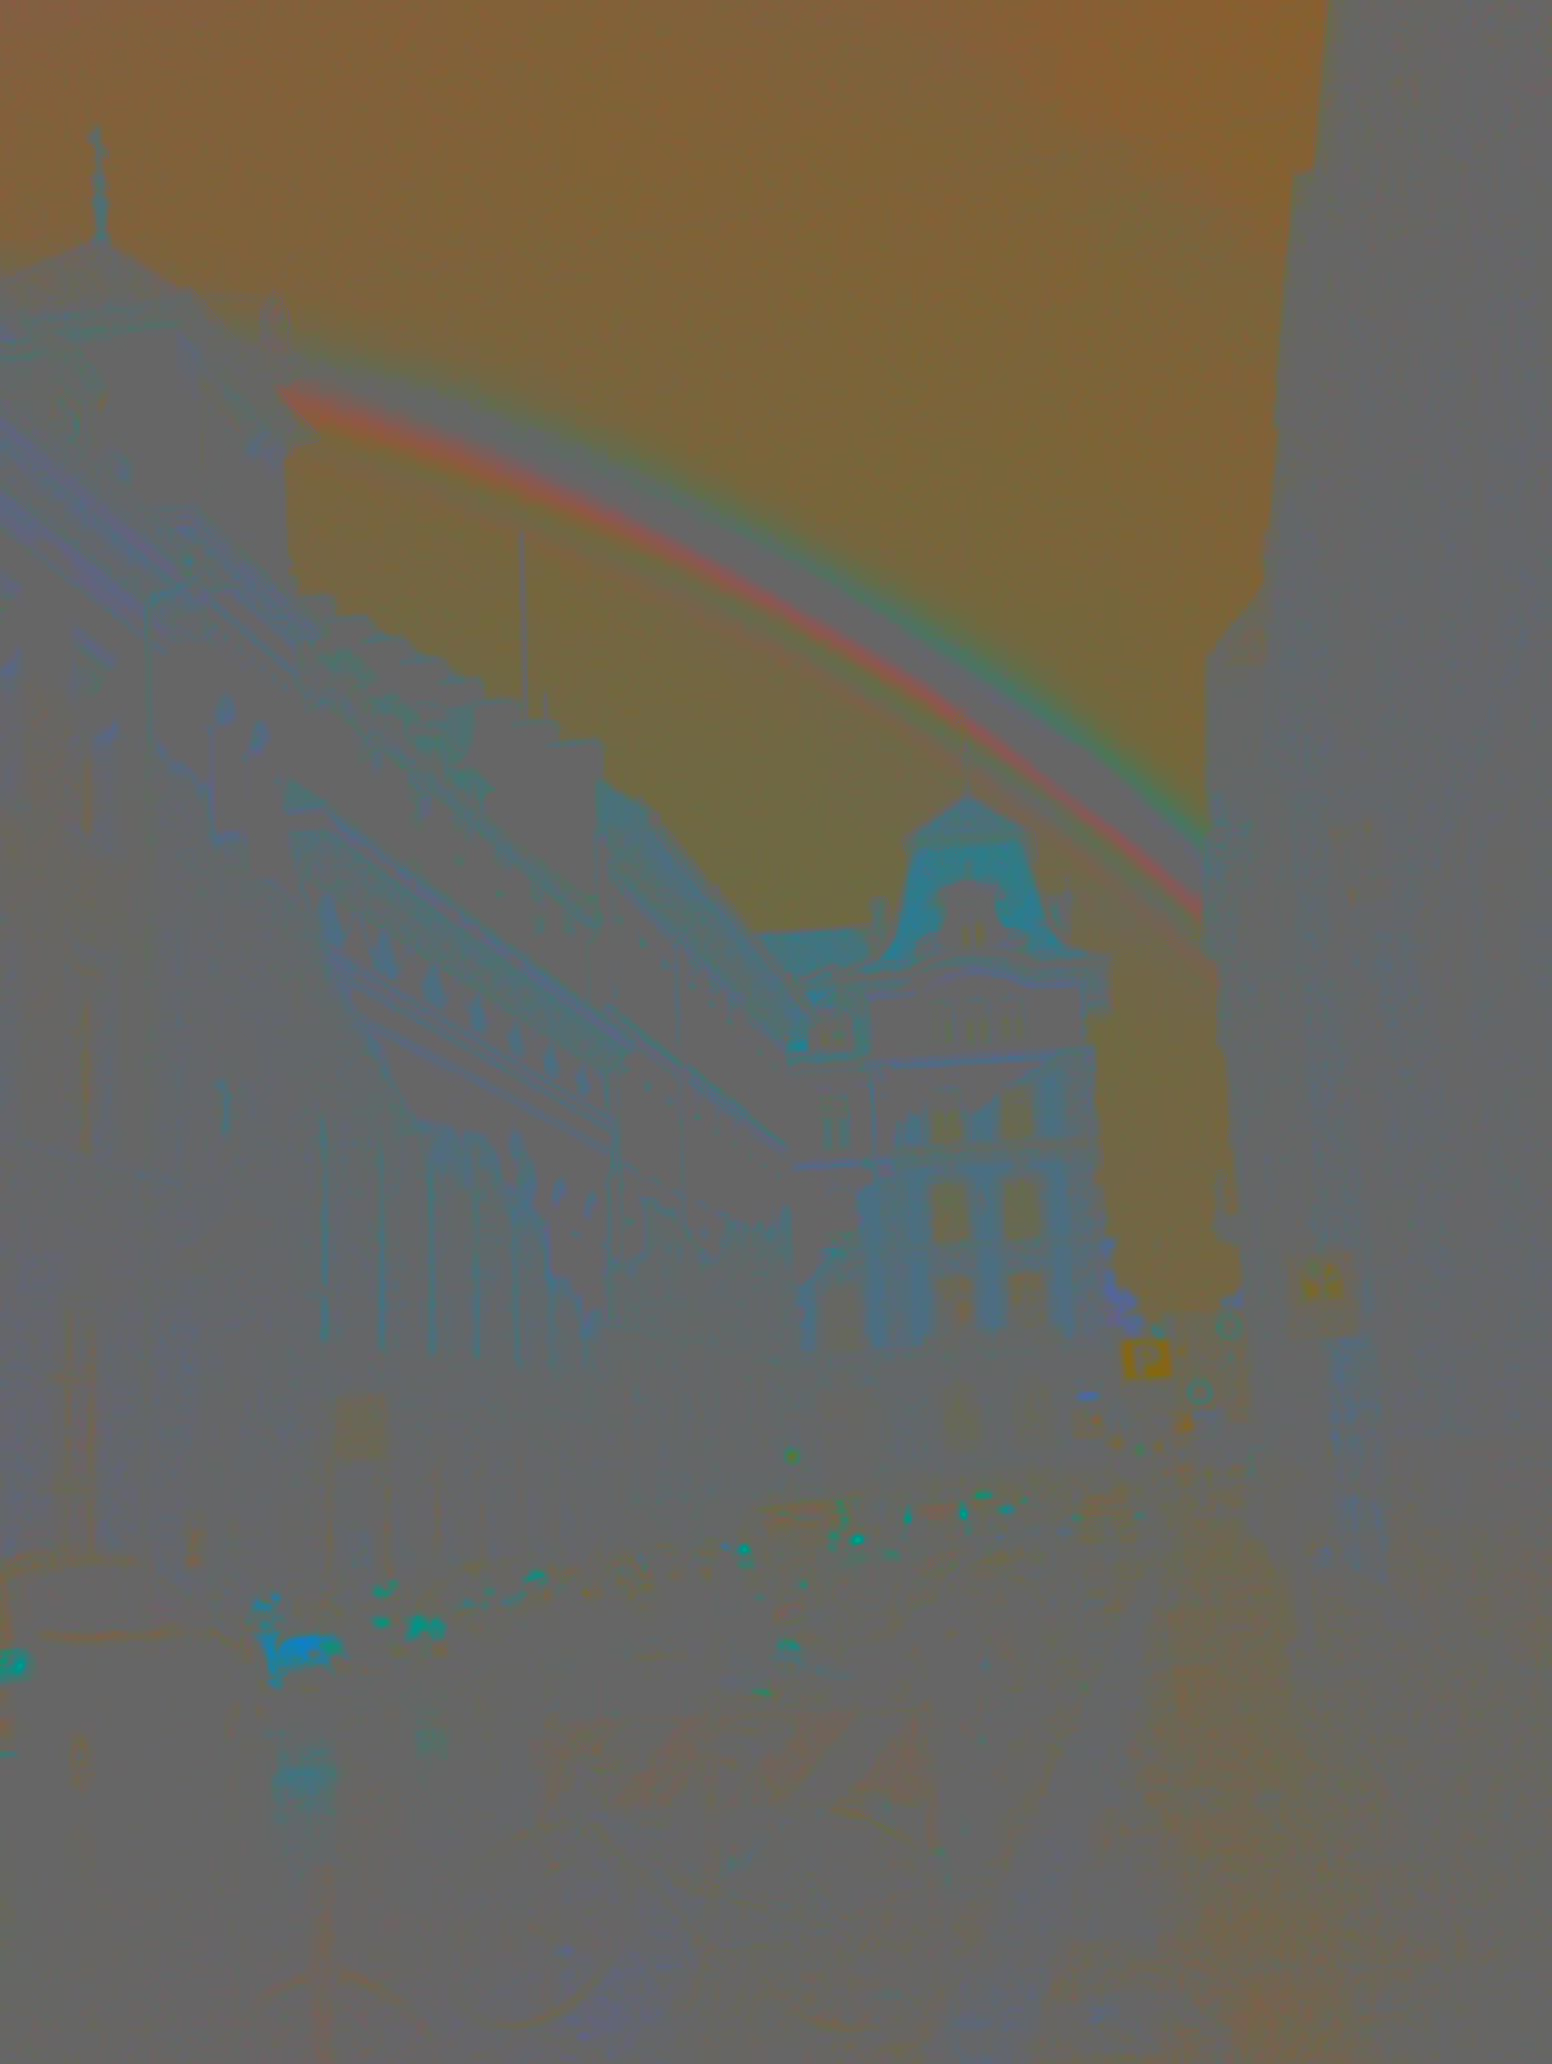
\includegraphics[width=\textwidth]{rainbow_inv}
		\caption*{Inverted image}
	\end{subfigure}
	~
	\begin{subfigure}[h]{0.48\textwidth}
		\centering
		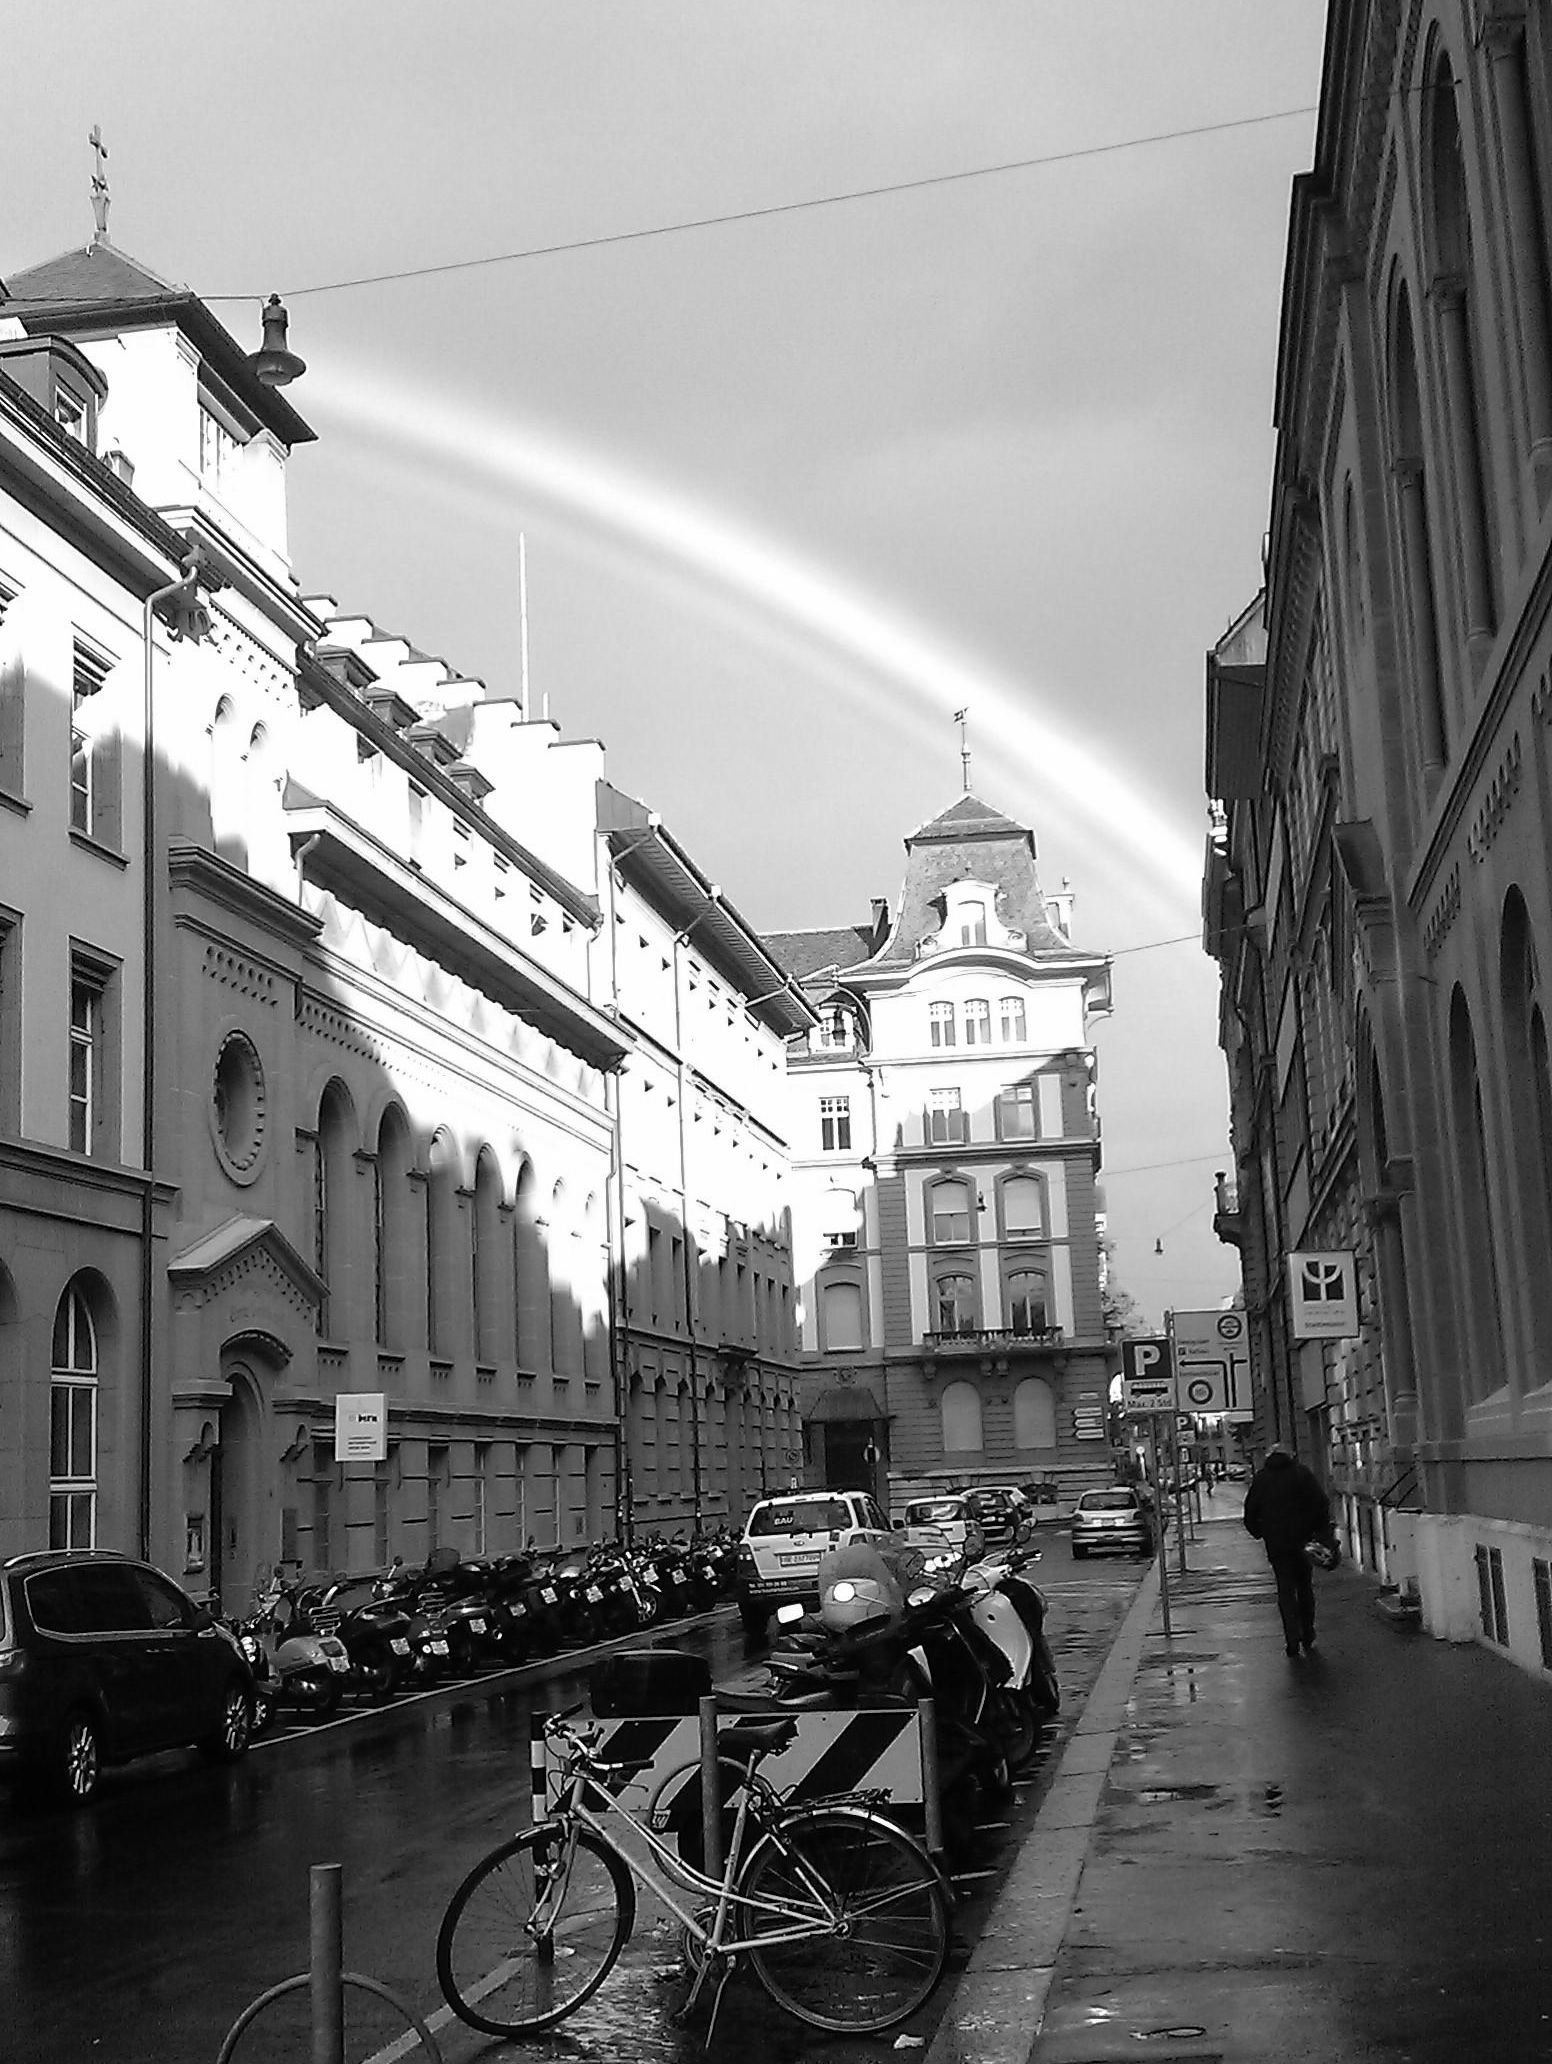
\includegraphics[width=\textwidth]{rainbow_gray}
		\caption*{Gray-scale image}
	\end{subfigure}	
\caption{The spanish castle illusion with the example of a photograph with a rainbow captured in Bern in September 2013. Starring at the inverted image long enough and then at the gray-scale image will produce the astonishing effect of perceiving the original colors in the gray-scale image.}
\label{fig:rainbow}
\end{figure}

\begin{figure}[H]
	%\centering
	\begin{subfigure}[h]{0.24\textwidth}
		\centering
		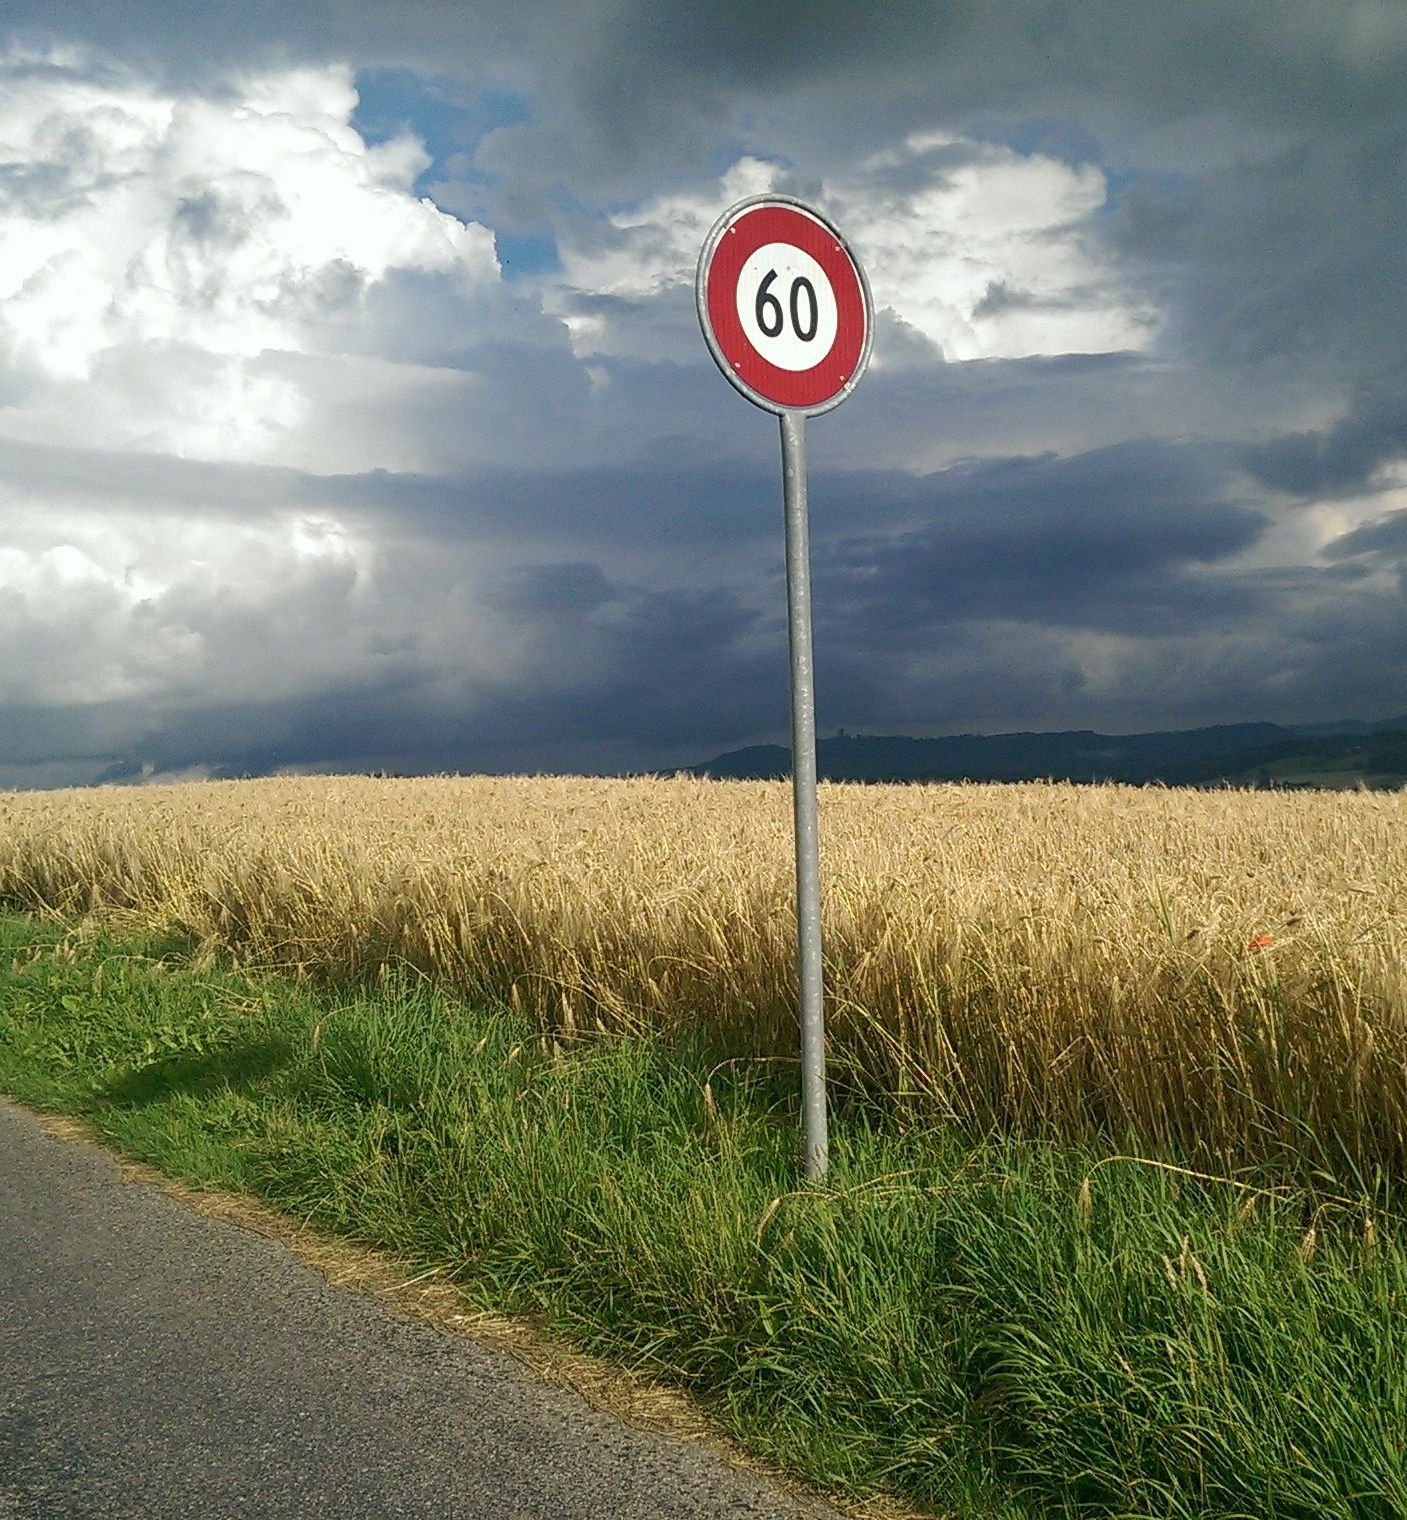
\includegraphics[width=\textwidth]{road}
		\caption*{Input image}
	\end{subfigure}
	
	\vspace{3mm}
	\begin{subfigure}[h]{0.48\textwidth}
		\centering
		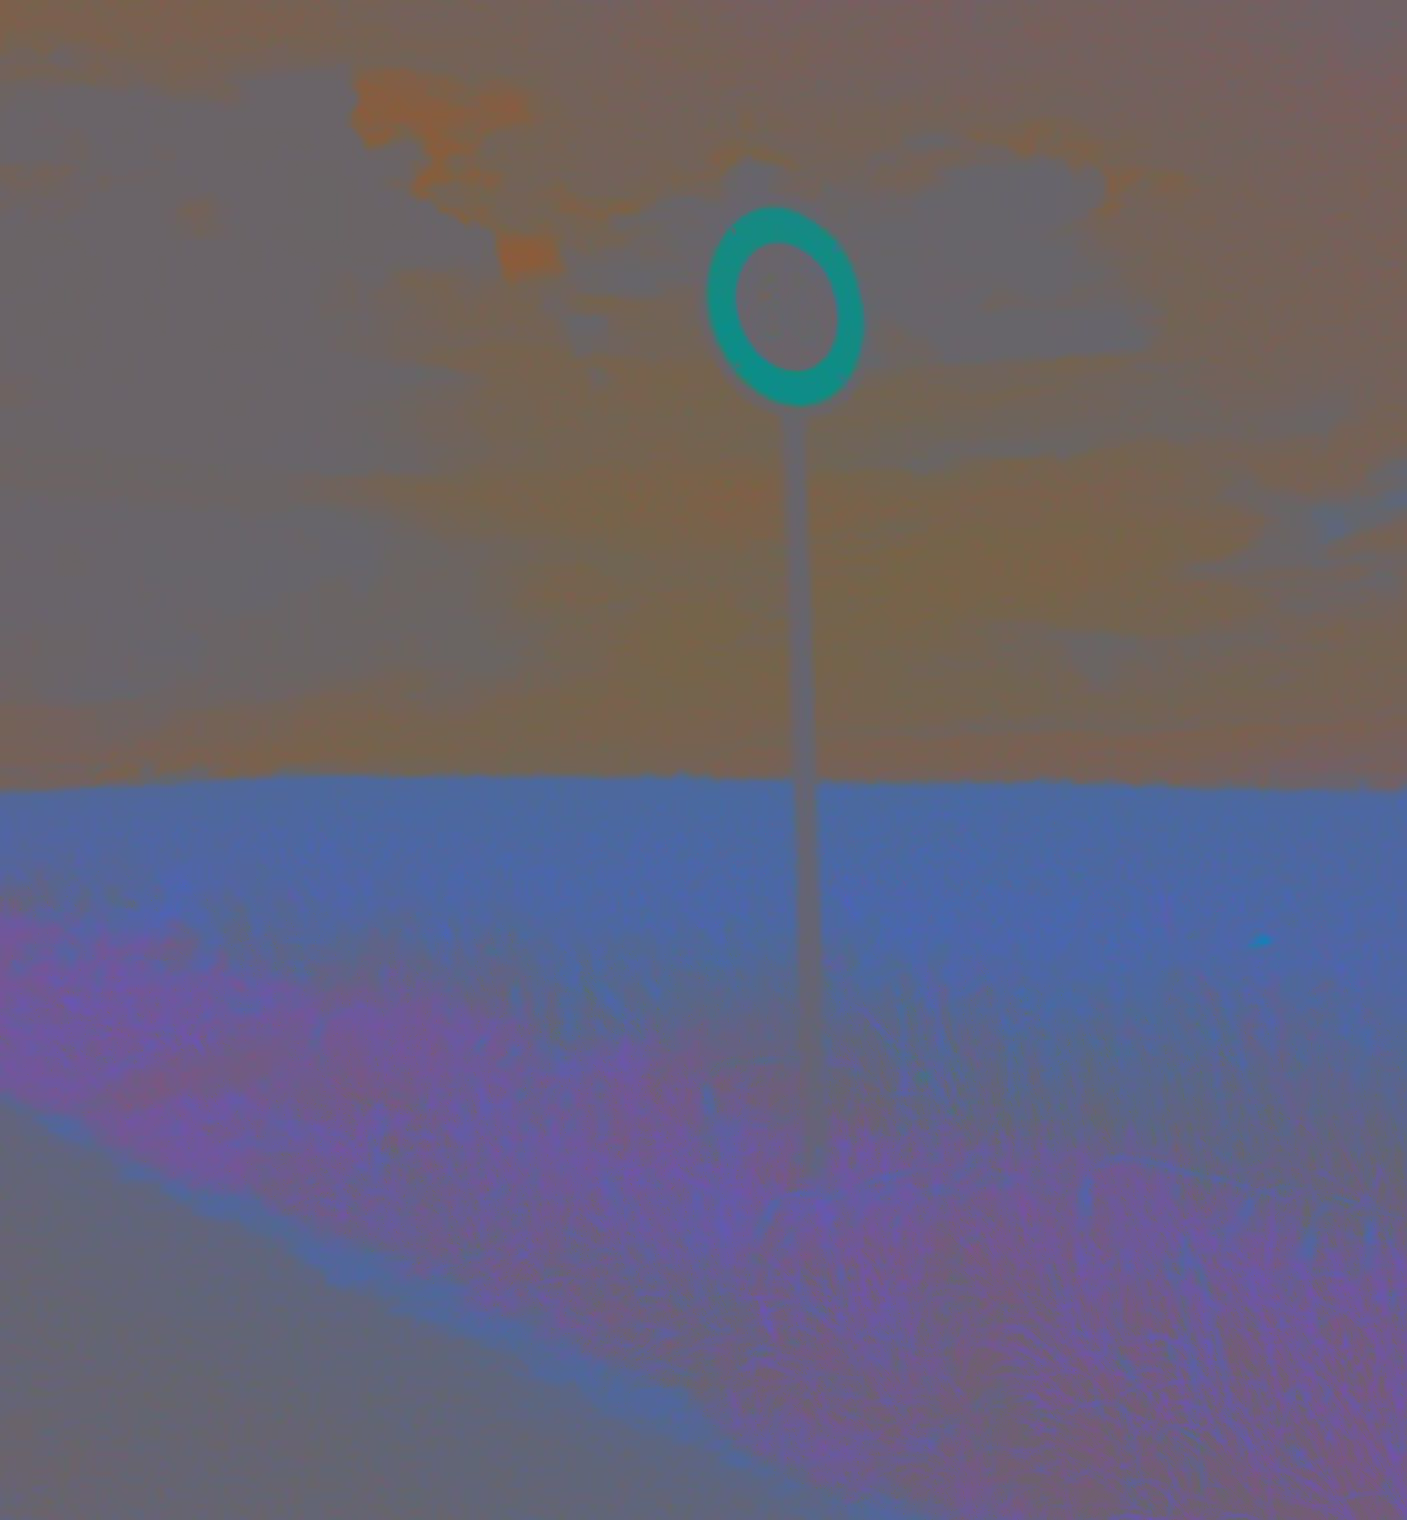
\includegraphics[width=\textwidth]{road_inv}
		\caption*{Inverted image}
	\end{subfigure}
	~
	\begin{subfigure}[h]{0.48\textwidth}
		\centering
		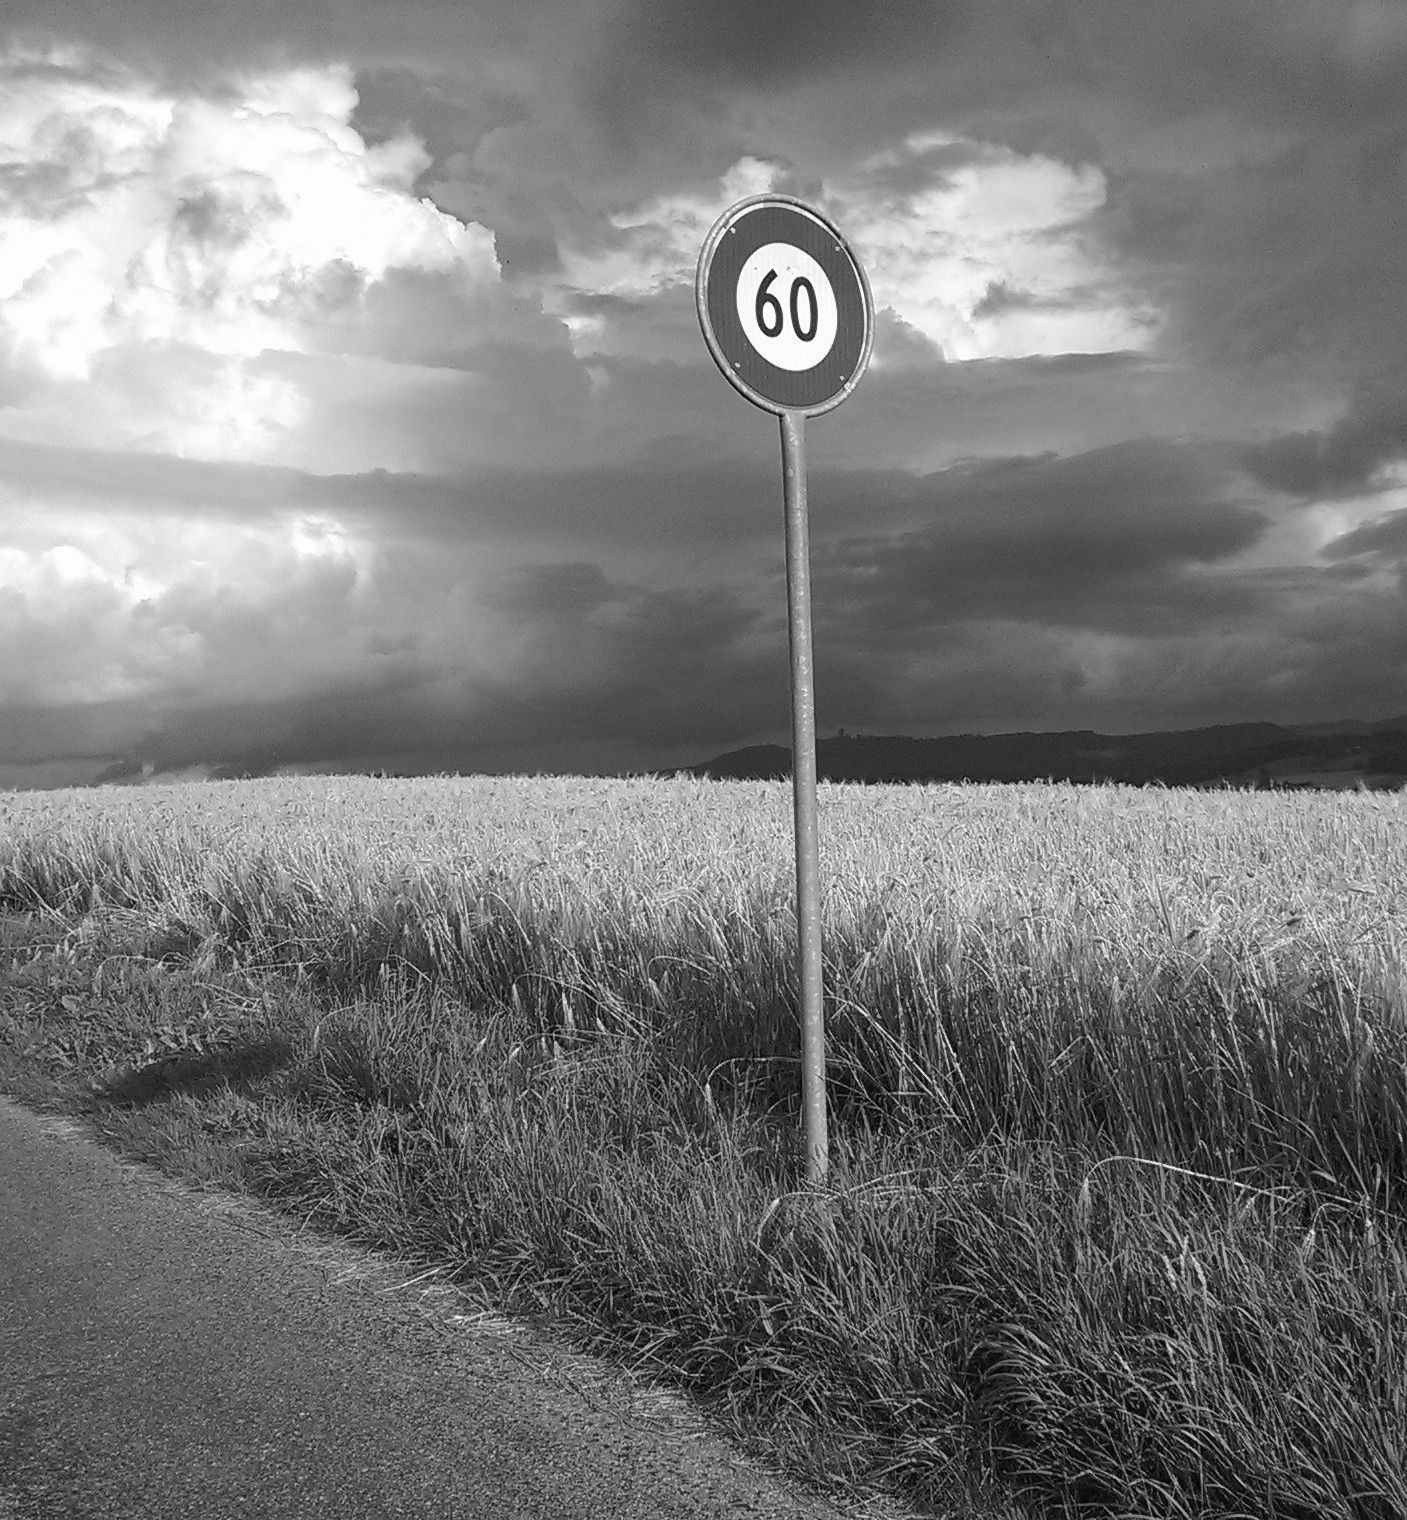
\includegraphics[width=\textwidth]{road_gray}
		\caption*{Gray-scale image}
	\end{subfigure}	
\caption{The spanish castle illusion with the example of a photograph captured near Bern in July 2014.}
\label{fig:road}
\end{figure}

\begin{figure}[H]
	%\centering
	\begin{subfigure}[h]{0.24\textwidth}
		\centering
		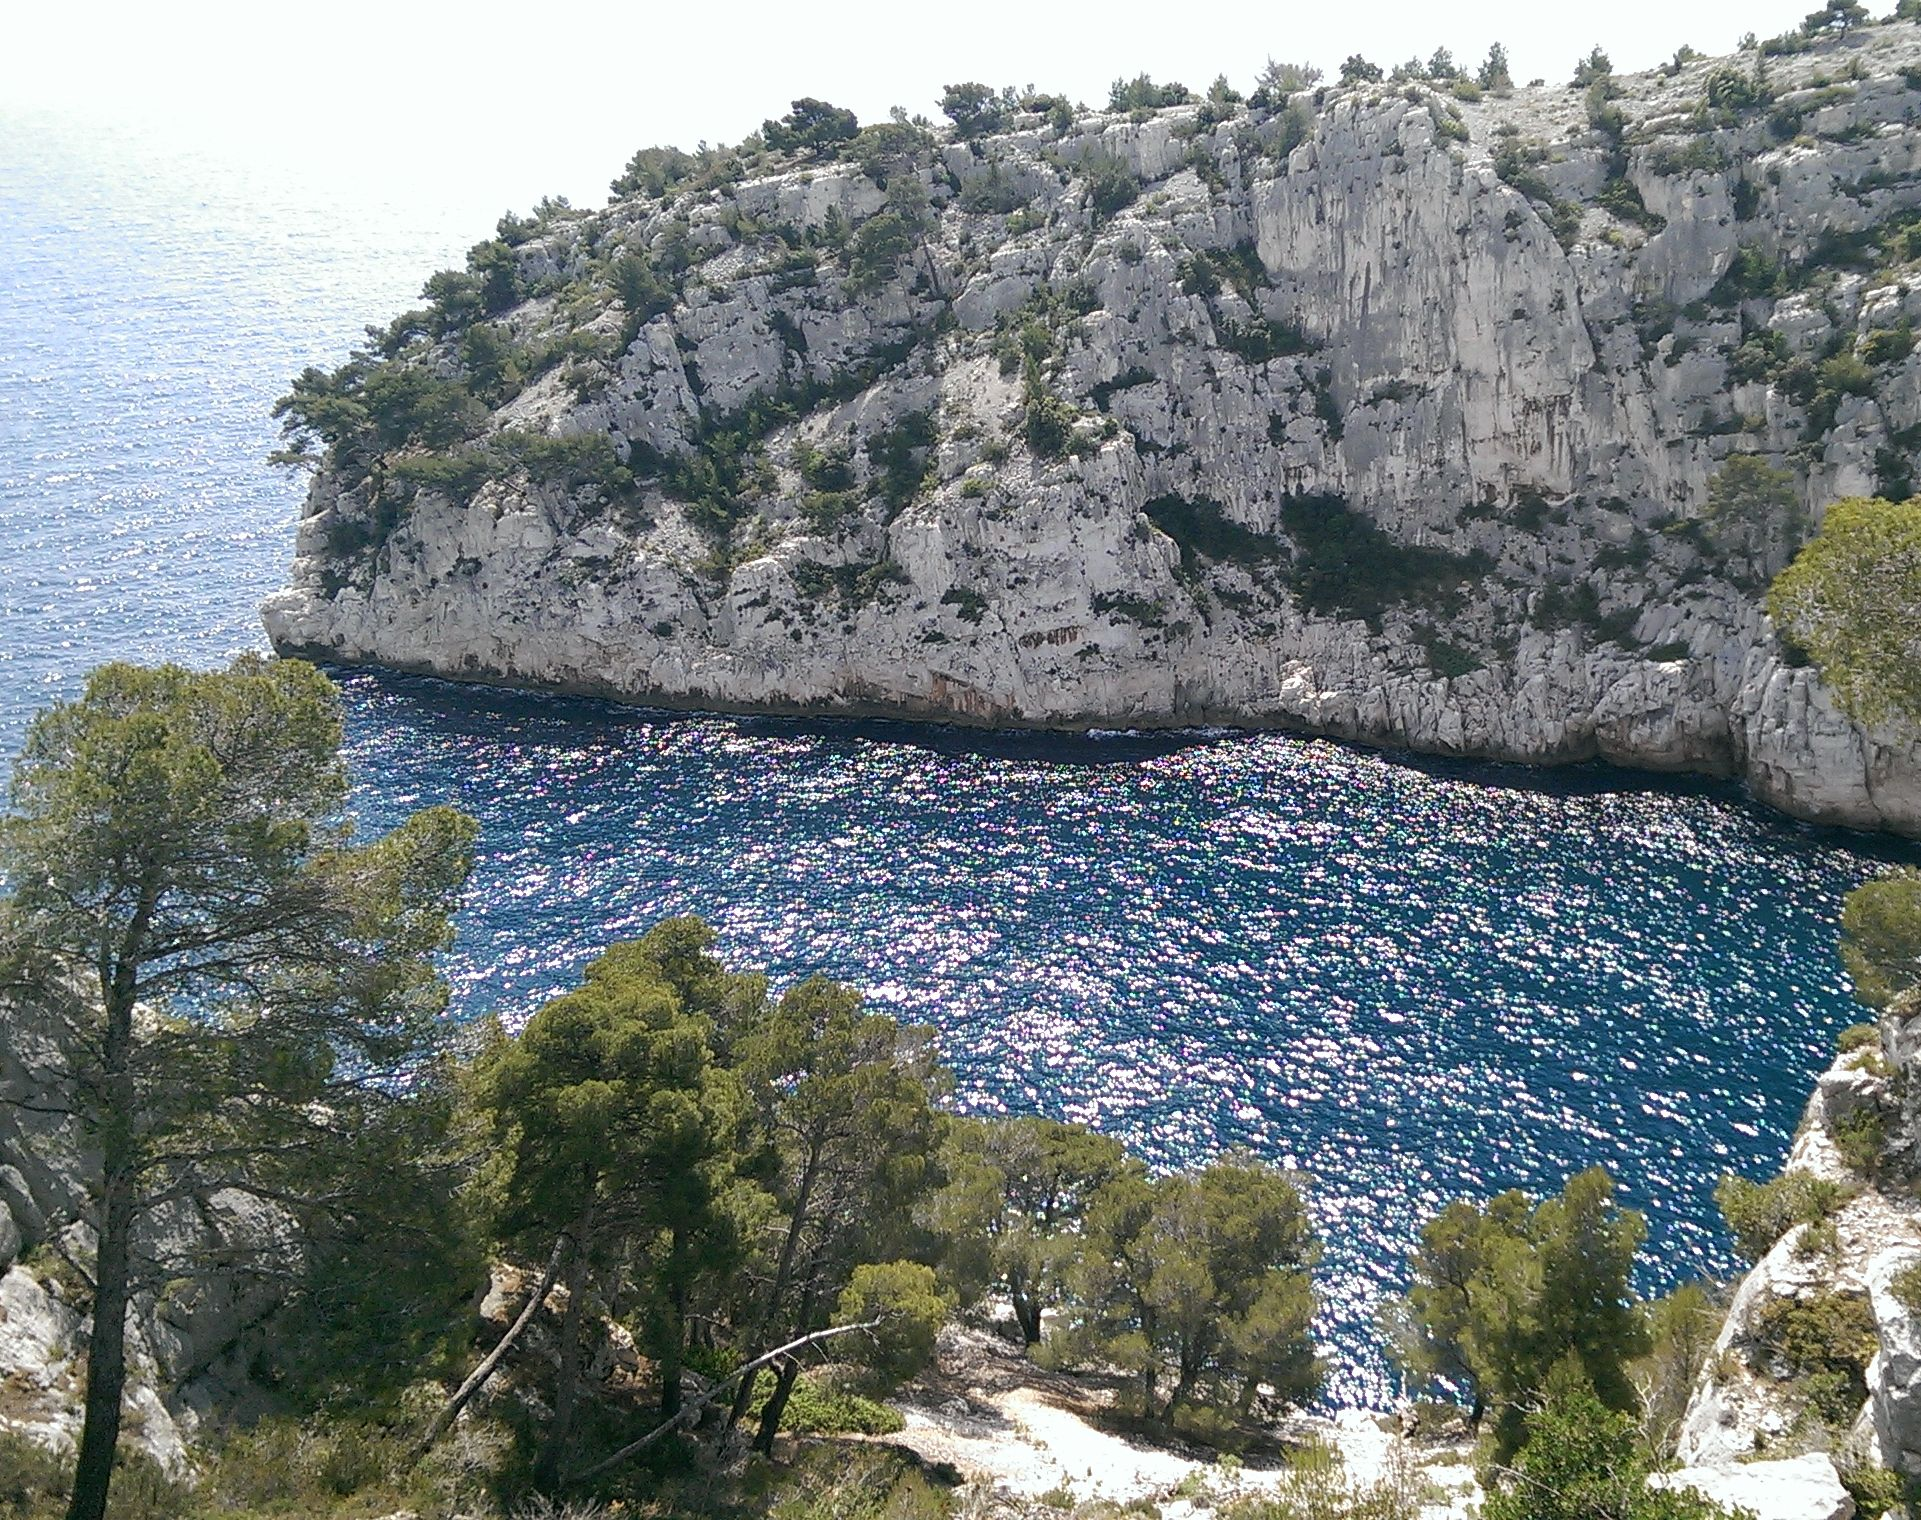
\includegraphics[width=\textwidth]{calanque}
		\caption*{Input image}
	\end{subfigure}
	
	\vspace{3mm}
	\begin{subfigure}[h]{0.48\textwidth}
		\centering
		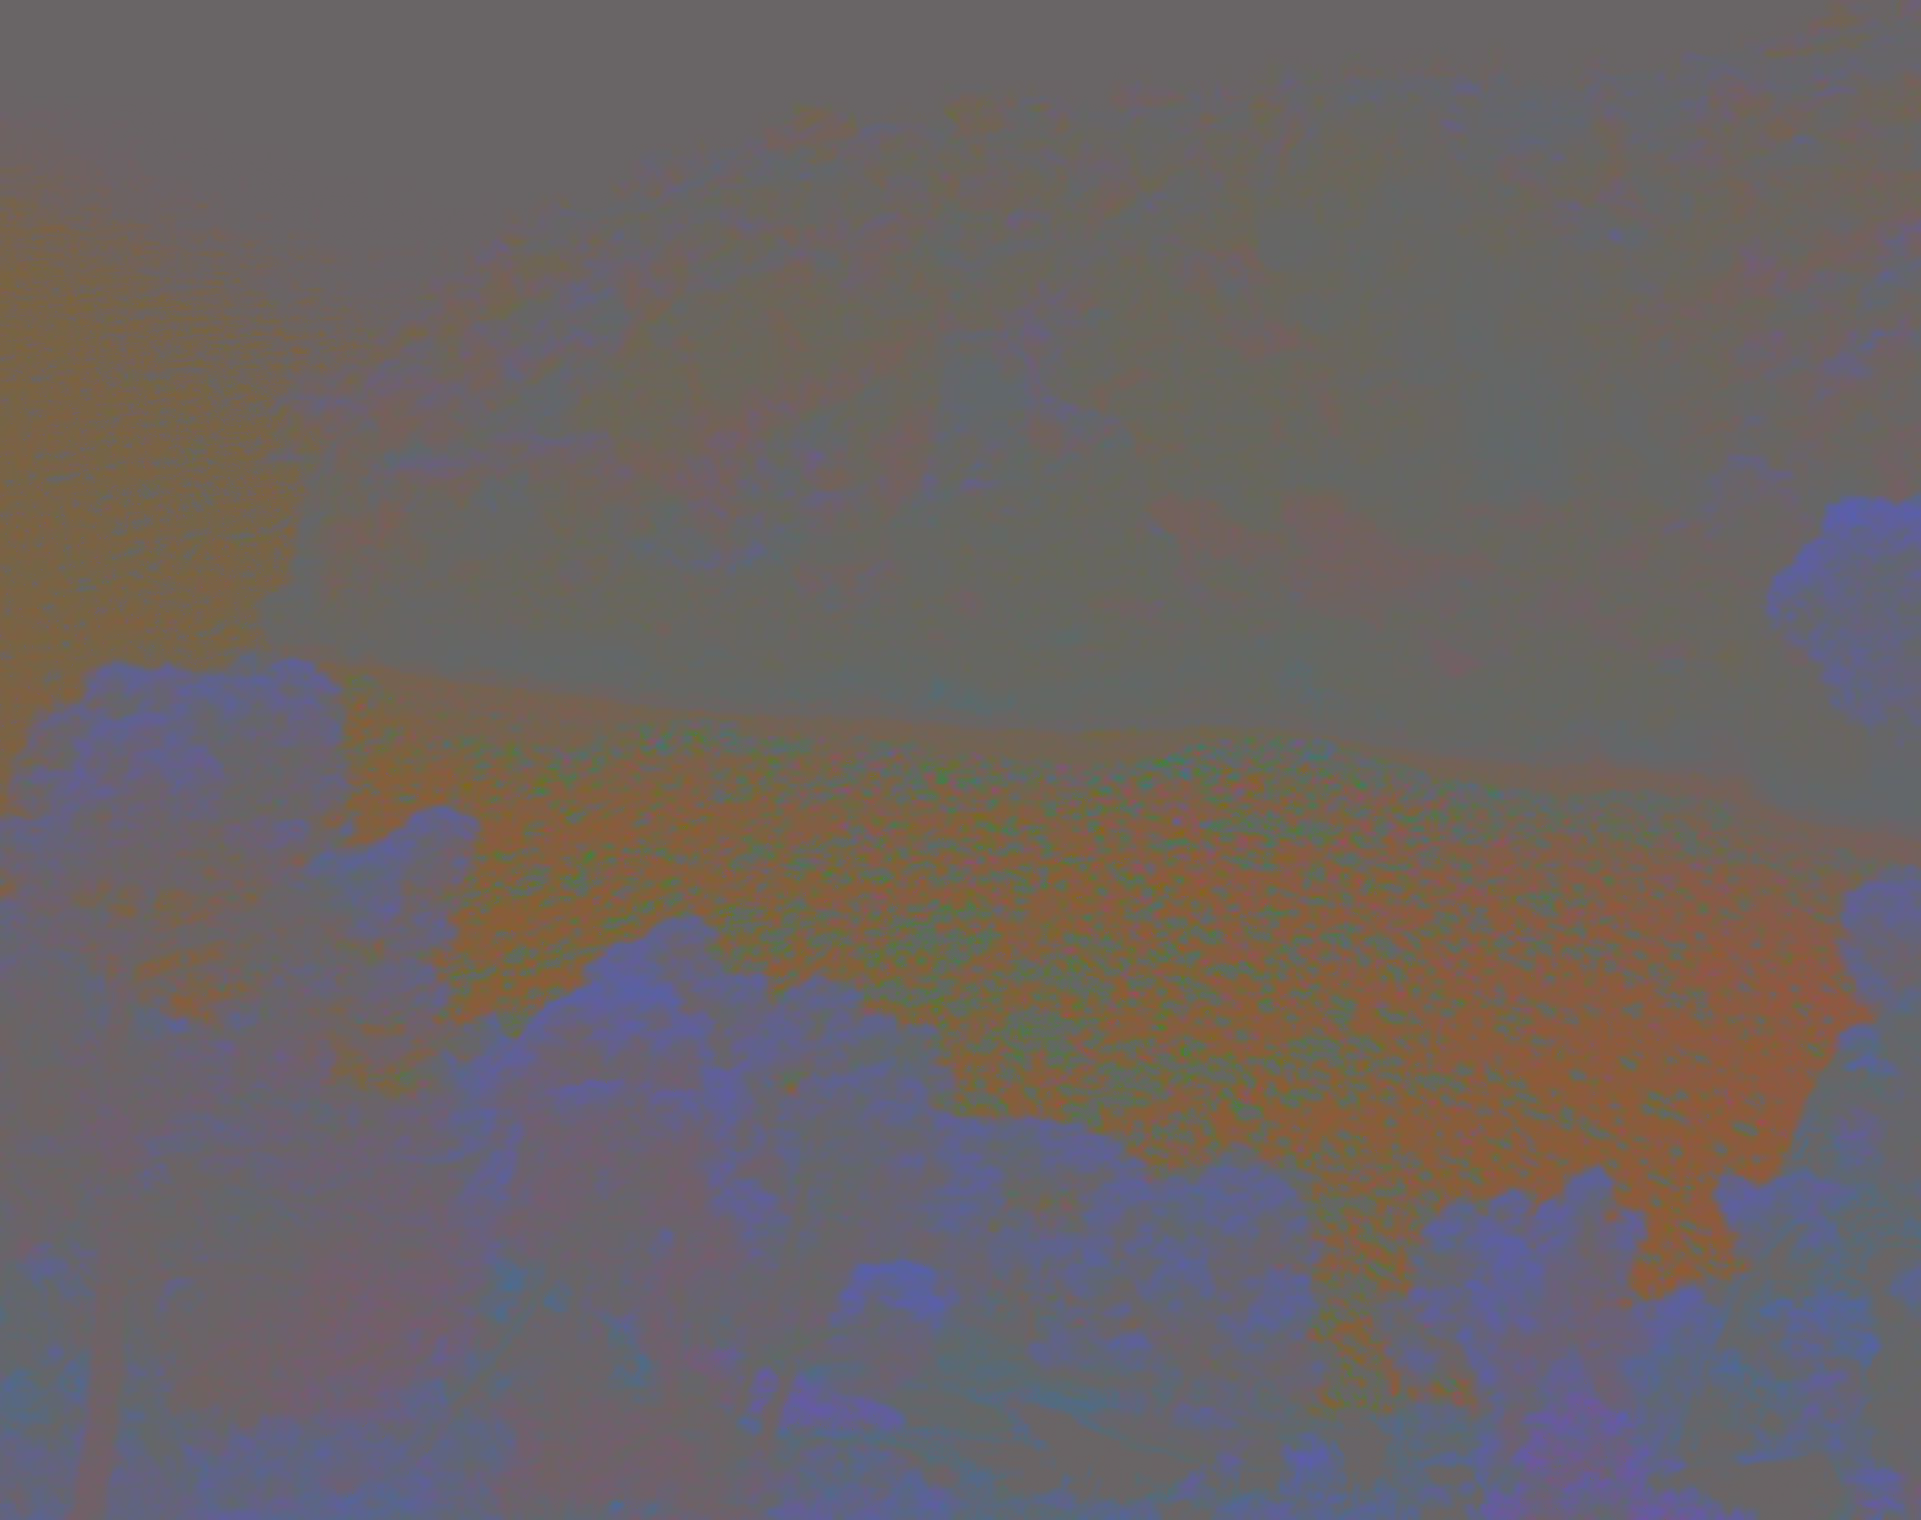
\includegraphics[width=\textwidth]{calanque_inv}
		\caption*{Inverted image}
	\end{subfigure}
	~
	\begin{subfigure}[h]{0.48\textwidth}
		\centering
		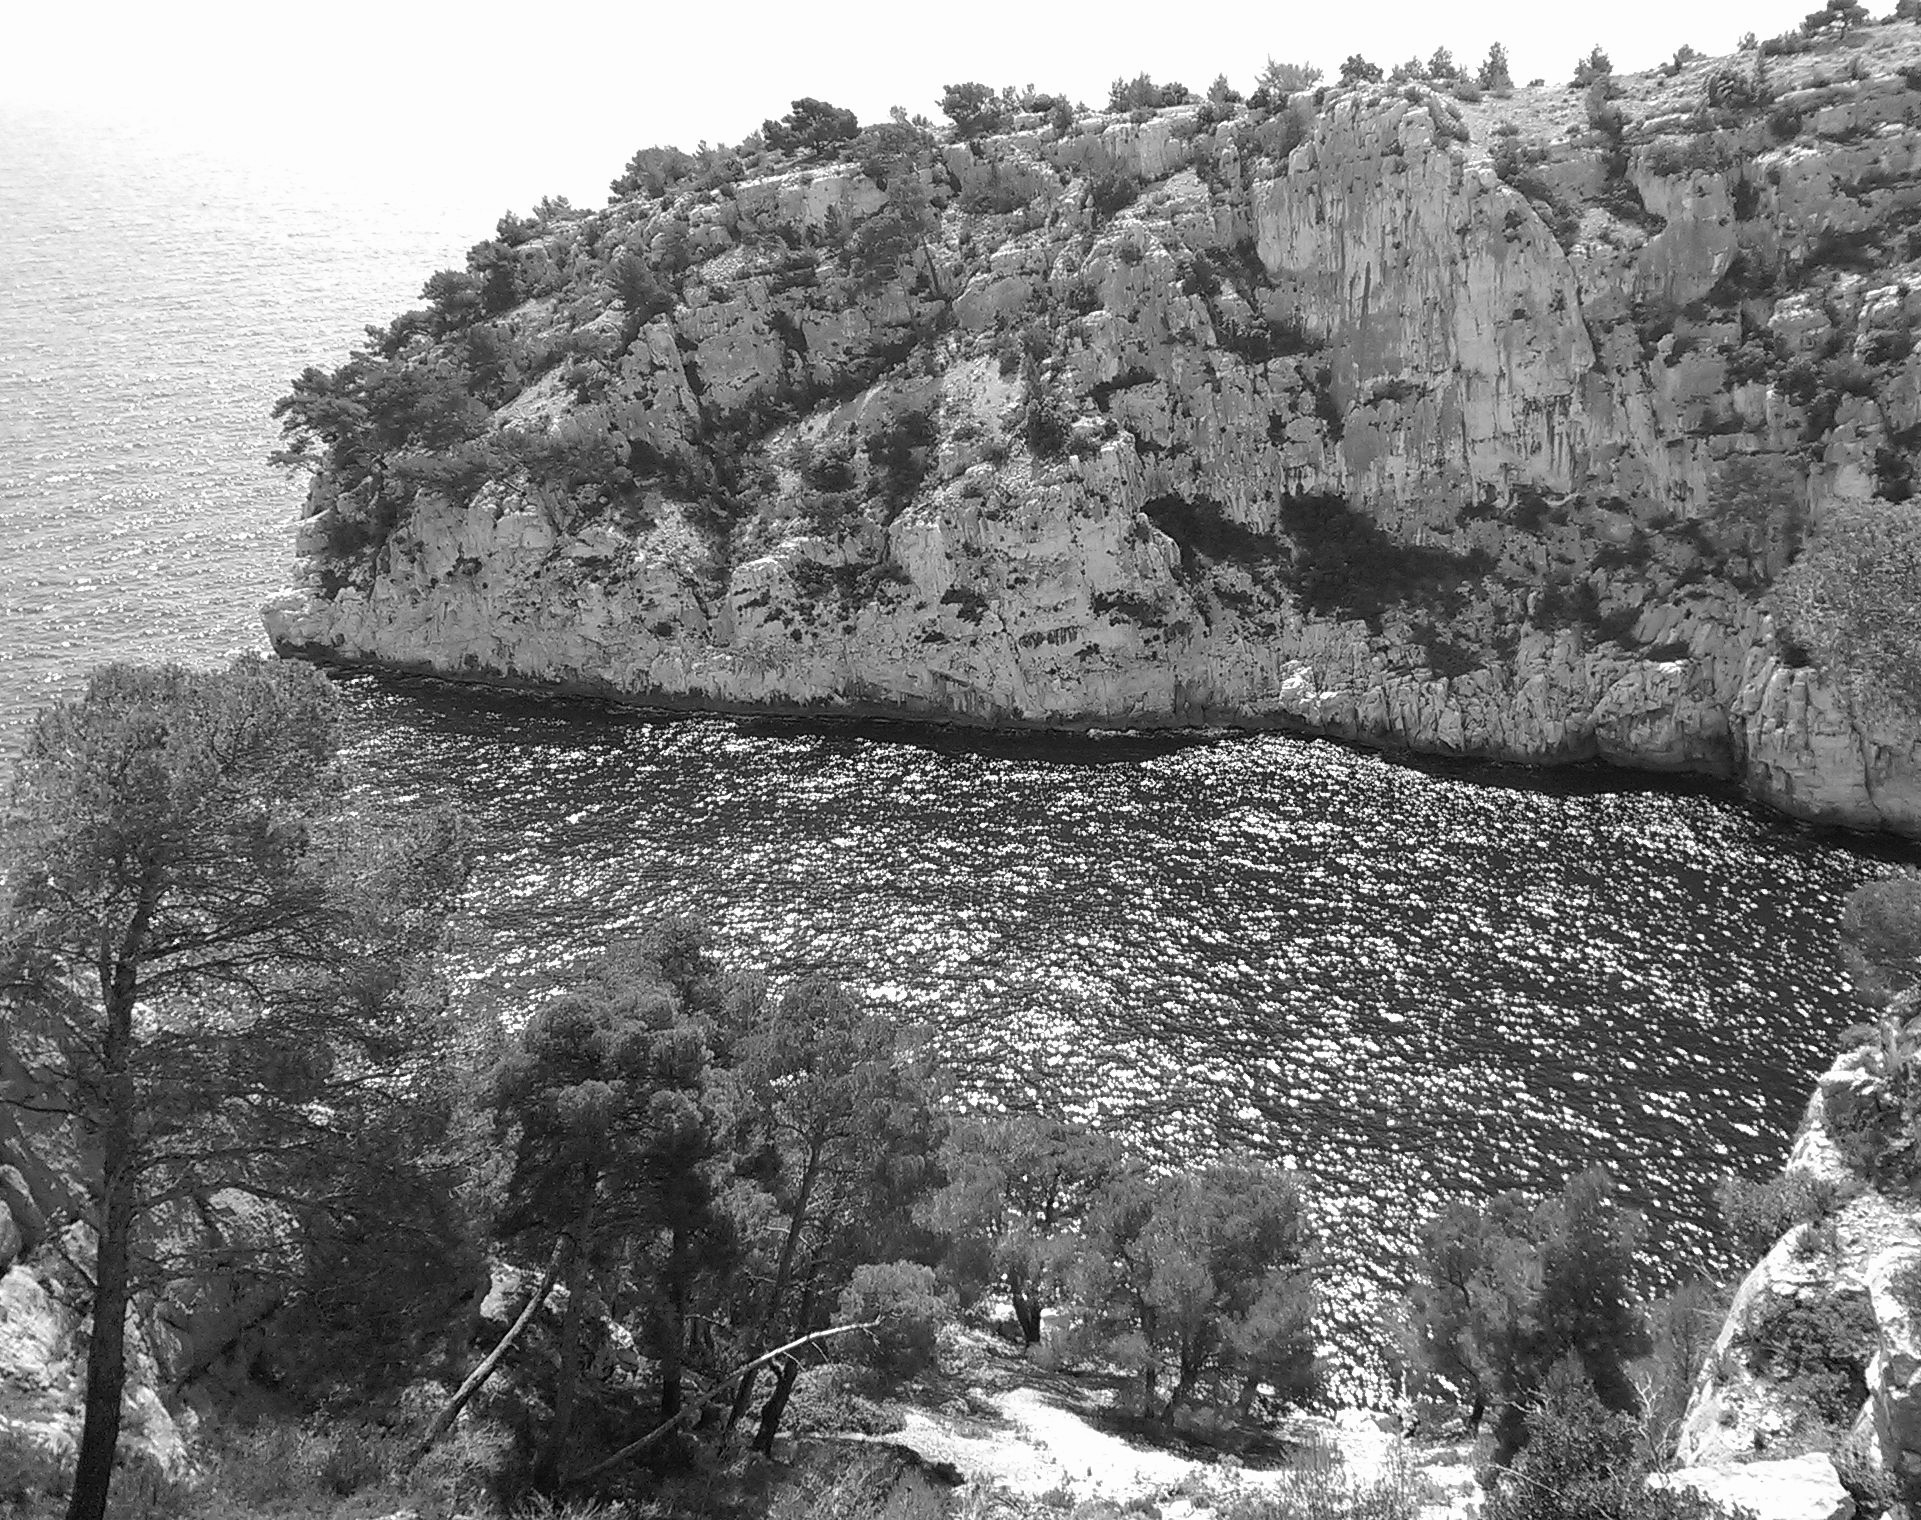
\includegraphics[width=\textwidth]{calanque_gray}
		\caption*{Gray-scale image}
	\end{subfigure}	
\caption{The spanish castle illusion with the example of a photograph captured near Cassis in May 2014.}
\label{fig:calanque}
\end{figure}

\section{Processing RAW Images}
\begin{figure}[H]
	\centering
	\vspace{3mm}
	\begin{subfigure}[h]{0.48\textwidth}
		\centering
		\includegraphics[width=\textwidth]{raw_forest_input}
		\caption*{Input}
	\end{subfigure}
	~
	\begin{subfigure}[h]{0.48\textwidth}
		\centering
		\includegraphics[width=\textwidth]{raw_forest_demosaiced_linear}
		\caption*{Demosaiced}
	\end{subfigure}	
\caption{Left: Input RAW data. Every pixel only contains the red, green or blue value, but never more than one. Therefore it can be represented by a gray-scale image. Right: Reconstructed (demosaiced) RGB image through bilinear filtering.}
\label{fig:demosaicLin}
\end{figure}

\begin{figure}[H]
	\centering
	\begin{subfigure}[h]{0.48\textwidth}
		\centering
		
\includegraphics[width=\textwidth]{black_and_white_bilinear_interpolated}
		\caption*{Bilinear interpolation}
	\end{subfigure}
	~
	\begin{subfigure}[h]{0.48\textwidth}
		\centering
		
\includegraphics[width=\textwidth]{black_and_white_median_filtered_3x3}
		\caption*{3x3 median filtered}
	\end{subfigure}	
	
	\vspace{3mm}
	\centering
	\begin{subfigure}[h]{0.32\textwidth}
		\centering
		
\includegraphics[width=\textwidth]{black_and_white_bilinear_interpolated_zoom}
		\caption*{Zoom bilinear}
	\end{subfigure}
	\begin{subfigure}[h]{0.32\textwidth}
		\centering
		
\includegraphics[width=\textwidth]{black_and_white_median_filtered_3x3_zoom}
		\caption*{Zoom 3x3 median}
	\end{subfigure}
	\begin{subfigure}[h]{0.32\textwidth}
		\centering
		
\includegraphics[width=\textwidth]{black_and_white_median_filtered_5x5_zoom}
		\caption*{Zoom 5x5median}
	\end{subfigure}
\caption{Comparison between bilinear interpolation and median filtering.}
\label{fig:calanque}
\end{figure}
\todo{Write something, maybe do cool plots}
\section{Color Balancing}

\end{document}